\documentclass[12pt]{standalone}
\usepackage{tikz}
%\usetikzlibrary{calc, arrows.meta, decorations.pathreplacing}

\begin{document}


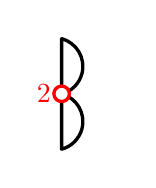
\begin{tikzpicture}[line width=1.2pt, line cap=round, line join=round, scale=1.4]
		\begin{scope}[even odd rule]
\clip (-0.1, -0.1) rectangle (0.6, 1.1) (0,0.5) circle(2pt);
       \draw (0,0) -- (0,1) arc[start angle=75, end angle=-75, radius=0.26] -- (0,0.5) arc[start angle=75, end angle=-75, radius=0.26] -- (0,0);
		\end{scope}
			\draw[red] (0, 0.5) circle(2pt) node[anchor=east]{2};
	\end{tikzpicture}
\end{document}
